\documentclass[a4paper,12pt]{jsarticle}
\usepackage[T1]{fontenc}
\usepackage{newenum}
\usepackage{epsfig}

\usepackage{enumerate}

\usepackage{graphicx}
\newcommand{\figdir}{../figures}

% theorem
\usepackage{amsmath,amssymb}
\usepackage{amsthm}
\newtheorem*{cooperativepatrollingproblem}{{\patProb}}
\newtheorem*{timeSpecifiedCooperativePatrollingProblem}{時刻指定{\patProb}}
\newtheorem*{timeSpecifiedCooperativePatrollingProblemDecision}{時刻指定協力警邏判定問題}
\newtheorem*{timeSpecifiedProblemOnLine}{時刻指定線分警邏問題}
\newtheorem*{timeSpecifiedProblemOnLineSubProb}{副問題}
\newtheorem*{greedyAlgorithmForTimeSpecifiedProblemOnLine}{貪欲アルゴリズム}


 % Tikz
	\usepackage[dvipdfmx,svgnames]{xcolor}%tikzパッケージよりも前に読み込みます。
	\usepackage{tikz}%(これで,pgf と pgffor も読み込まれます。)
%%% color %%%
	% \usepackage[dvipdfmx]{color}    % 色付き文字
	\definecolor{mygreen}{rgb}{0, 0.6, 0} % R(赤),G(緑),B(青)
	\definecolor{myorange}{rgb}{0.8, 0.4, 0} % R(赤),G(緑),B(青)
	\newcommand{\black}      [1] {{\textcolor{black}{#1}}}
	\newcommand{\red}        [1] {{\textcolor{red}{#1}}}
	\newcommand{\blue}       [1] {{\textcolor{blue}{#1}}}
	\newcommand{\green}      [1] {{\textcolor{mygreen}{#1}}}
	\newcommand{\orange}     [1] {{\textcolor{myorange}{#1}}}


\def\newblock{\hskip .11em plus .33em minus .07em}

\newcommand{\optpp}      {O{\scriptsize PTIMIZE}PP}
\newcommand{\decisionpp} {D{\scriptsize ECISION}PP}
\newcommand{\timelimit}  {許容訪問間隔}
\newcommand{\period}     {厳密訪問間隔}
\newcommand{\comp}       {Comp}





%%%%% 定義環境 %%%%%
	\theoremstyle{definition}
	\newtheorem {theo}          {定理}[section]
	\newtheorem {defi}[theo]    {定義}
	\newtheorem {prop}[theo]    {命題}
	\newtheorem {lemm}[theo]    {補題}
	\newtheorem {coro}[theo]    {系} % corollary
	\newtheorem {conj}[theo]    {予想} % conjecture
	% \newtheorem*{note}          {注意}
	\newtheorem*{rema}          {Remark}
	\newtheorem*{exam}          {例}
	\newtheorem*{exer}          {例題}
	\newtheorem*{memo}          {メモ}
	\newtheorem*{property}      {性質}


%%% newcommand
	\newcommand{\Ref}        [1]{{(\ref{#1})}}
	\newcommand{\wc}            {{}\cdot{}}

	\newcommand{\dbigcup}       {\bigcup\limits}
	\newcommand{\dbigcap}       {\bigcap\limits}
	\newcommand{\dsum}          {\sum\limits}
	\newcommand{\dmax}          {\max\limits}
	\newcommand{\dmin}          {\min\limits}
	\newcommand{\dsup}          {\sup\limits}
	\newcommand{\dinf}          {\inf\limits}
	\newcommand{\dprod}         {\prod\limits}

	\newcommand{\set}        [1]{\left\{{#1}\right\}}
	\newcommand{\setmid}     [2]{\left\{{#1}\;\middle|\;{#2}\right\}}  %% intension
	\newcommand{\frc}        [1]{\frac{1}{#1}}
	\newcommand{\sforall}       {{}^\forall}
	\newcommand{\sexists}       {{}^\exists}
	\newcommand{\N}             {\mathbb{N}}
	\newcommand{\Z}             {\mathbb{Z}}
	\newcommand{\R}             {\mathbb{R}}
	\newcommand{\bigland}       {\bigwedge}
	\newcommand{\biglor}        {\bigvee}
	\newcommand{\AND}           {\quad\text{and}\quad}
	\newcommand{\OR}            {\quad\text{or}\quad}
	\newcommand{\IF}            {\quad\text{if}\quad}
	\newcommand{\ELSE}          {\quad\text{else}\quad}
	\newcommand{\OTHERWISE}     {\quad\text{otherwise}\quad}
%%% 矢印 %%%
	\newcommand{\To}            {{\;\Rightarrow\;}}
	\newcommand{\Gets}          {{\;\Leftarrow\;}}
	\newcommand{\Iff}           {{\;\Leftrightarrow\;}}
 % (x)
	\newcommand{\lr}         [1]{\left(#1\right)}
	\newcommand{\bigkakko}   [1]{\bigl(#1\bigr)}
	\newcommand{\Bigkakko}   [1]{\Bigl(#1\Bigr)}
	\newcommand{\biggkakko}  [1]{\biggl(#1\biggr)}
	\newcommand{\Biggkakko}  [1]{\Biggl(#1\Biggr)}
 % {x}
	\newcommand{\lrbrace}    [1]{\left\{#1\right\}}
	\newcommand{\bigbrace}   [1]{\bigl\{#1\bigr\}}
	\newcommand{\Bigbrace}   [1]{\Bigl\{#1\Bigr\}}
	\newcommand{\biggbrace}  [1]{\biggl\{#1\biggr\}}
	\newcommand{\Biggbrace}  [1]{\Biggl\{#1\Biggr\}}
 % [x]
	\newcommand{\lrbrack}    [1]{\left[{#1}\right]}
	\newcommand{\bigbrack}   [1]{\bigl[{#1}\bigr]}
	\newcommand{\Bigbrack}   [1]{\Bigl[{#1}\Bigr]}
	\newcommand{\biggbrack}  [1]{\biggl[{#1}\biggr]}
	\newcommand{\Biggbrack}  [1]{\Biggl[{#1}\Biggr]}
 % |x|
	\newcommand{\abs}        [1]{|{#1}|}
	\newcommand{\lrabs}      [1]{\left|{#1}\right|}
	\newcommand{\bigabs}     [1]{\bigl|{#1}\bigr|}
	\newcommand{\Bigabs}     [1]{\Bigl|{#1}\Bigr|}
	\newcommand{\biggabs}    [1]{\biggl|{#1}\biggr|}
	\newcommand{\Biggabs}    [1]{\Biggl|{#1}\Biggr|}
 % <x>
	\newcommand{\nangle}     [1]{\langle{#1}\rangle}
	\newcommand{\lrangle}    [1]{\left\langle{#1}\right\rangle}
	\newcommand{\bigangle}   [1]{\bigl\langle{#1}\bigr\rangle}
	\newcommand{\Bigangle}   [1]{\Bigl\langle{#1}\Bigr\rangle}
	\newcommand{\biggangle}  [1]{\biggl\langle{#1}\biggr\rangle}
	\newcommand{\Biggangle}  [1]{\Biggl\langle{#1}\Biggr\rangle}
 % ||x||
	\newcommand{\norm}       [1]{\lVert{#1}\rVert}
	\newcommand{\lrnorm}     [1]{\left\lVert{#1}\right\rVert}
	\newcommand{\bignorm}    [1]{\bigl\lVert{#1}\bigr\rVert}
	\newcommand{\Bignorm}    [1]{\Bigl\lVert{#1}\Bigr\rVert}
	\newcommand{\biggnorm}   [1]{\biggl\lVert{#1}\biggr\rVert}
	\newcommand{\Biggnorm}   [1]{\Biggl\lVert{#1}\Biggr\rVert}
 % \lceil x \rceil
	\newcommand{\lrceil}     [1]{\left\lceil{#1}\right\rceil}
	\newcommand{\ceil}       [1]{\lceil{#1}\rceil}
	\newcommand{\bigceil}    [1]{\bigl\lceil{#1}\bigr\rceil}
	\newcommand{\Bigceil}    [1]{\Bigl\lceil{#1}\Bigr\rceil}
	\newcommand{\biggceil}   [1]{\biggl\ceil{#1}\biggr\rceil}
	\newcommand{\Biggceil}   [1]{\Biggl\ceil{#1}\Biggr\rceil}
 % \lfloor x \rfloor
	\newcommand{\lrfloor}    [1]{\left\lfloor{#1}\right\rfloor}
	\newcommand{\floor}      [1]{\lfloor{#1}\rfloor}
	\newcommand{\bigfloor}   [1]{\bigl\lfloor{#1}\bigr\rfloor}
	\newcommand{\Bigfloor}   [1]{\Bigl\lfloor{#1}\Bigr\rfloor}
	\newcommand{\biggfloor}  [1]{\biggl\floor{#1}\biggr\rfloor}
	\newcommand{\Biggfloor}  [1]{\Biggl\floor{#1}\Biggr\rfloor}
%%%%%%%%%%%%%%%%%%%%%%%%%%%%%%%%%%%%%%%%%%%%%%%%%



\title{複数の巡査の協力による指定地点の警邏について\\
	{\normalsize Collaborative Patrolling of Designated Points on Graphs}}
\author{
		河村 彰星 \\ Akitoshi Kawamura \and
		能城 秀彬 \\ Hideaki Noshiro
	}
%% 	\affliate{
%% 		東京大学総合文化研究科 \\
%% 		The University of Tokyo, Graduate School of Arts and Sciences
%% }






\begin{document}

\maketitle

%\begin{abstract}
1人または複数の巡査が所与の領域を動き回り,その領域内のあらゆる場所を十分な頻度で訪問することで,これを守備,監督することを警邏という.

Coeneらは,辺の長さの与えられた無向グラフと各頂点の持つ利得・{\idletime},巡査の人数が与えられたとき,グラフの辺上を速さ1以下で動く1人または複数の巡査が,各頂点を訪問する間隔をその頂点の{\idletime}以内にしなければならない制約を満たしながら訪問し続けることで警備するとき,警備される頂点の利得の合計を最大化するような頂点部分集合を求める警邏問題を考えた.
しかし,Coeneらは巡査が複数の場合もどの頂点も高々1人の巡査により警備されるという仮定を加えていた.

本稿ではこの問題を取り上げ,複数の巡査が協力して警備する頂点があってもよいという設定で同じ問題を考える.
NP困難性や多項式時間アルゴリズムを示すのが難しかった部分については,{\idletime}の代わりに「厳密訪問間隔」を考え,頂点を最初に訪問した時刻からちょうど厳密訪問間隔ごとの時刻にその頂点は訪問されなければならないという問題や,さらに最初の訪問時刻も与えられる問題を考えて計算量クラスの評価を試みる.


% Coeneらは,
% 辺の長さの与えられた無向グラフと各頂点の持つ利得・{\idletime},巡査の人数が与えられたとき,
% 巡査がグラフ上を速さ1以下で動き頂点を訪問することで
% 警備できる頂点集合のうち,利得の合計を最大化するものを求める警邏問題を考えた.
% ある頂点を警備できているとは,
% どの連続した2回の訪問も間隔がその点の{\idletime}以内となるように
% 訪問し続けられることと定義される.
% グラフが
% Line(1つの線分上にすべての頂点があるグラフ)または
% Circle(Line の両端をつなぐ辺を足したグラフ)
% で巡査が1人の場合には多項式時間アルゴリズム,
% 星,木,一般の場合についてはNP困難性が示されている.
% 本稿ではこの問題を取り上げ,
% 多項式時間で解けるか否か未解決であった
% Line で巡査が複数の場合や,
% 既にNP困難性が示されている星よりも単純な,
% 星で枝の長さがすべて等しい図形(本稿では UStar と呼ぶことにする)について
% 詳しく調べることにする.
% そのままの問題設定では解決できなかった部分については,
% {\idletime}の代わりに厳密訪問間隔が与えられたときに,
% 最初の訪問時刻からその厳密訪問間隔ごとの時刻は必ず訪問しなければならないという問題,
% さらに最初の訪問時刻も与えられる問題も考える.
\end{abstract}



\section{はじめに}
所与の領域を1人または複数の巡査が動き回り,
その領域内の指定された場所を十分な頻度で訪れることを
警邏(patrolling)という\cite{chen2013fence, coene2011charlemagne, czyzowicz2011boundary}.


本稿では,与えられた距離空間$U$内を速さ$1$以下の巡査$m$人が動きまわることにより,
集合$V \subseteq U$に属する多くの点に十分な頻度で訪れるという目標を考える.
すなわち次のような問題である.

巡査$i \in \{1, \ldots, m\}$の$U$上の運行$a _i \colon \Rset \to U$とは,
各時刻$t \in \Rset$における位置$a _i (t) \in U$を定めるものであって,
任意の時刻$s$,$t \in \Rset$に対し$a _i (s)$と$a _i (t)$の距離が$\abs{s - t}$を超えないものをいう.
巡査$m$人による$U$上の運行とは,
全巡査の運行を定めた組
$A = (a _1, \dots, a _m)$をいう.
運行$A = (a _1, \dots, a _m)$
が点$v \in U$を{\idletime}$q \geq 0$で警備するとは,
長さ$q$のどの時間区間にも
いずれかの巡査が$v$を少くとも一度は訪れる
(任意の時刻$t \in \Rset$に対して
巡査$i$と時刻$\tau \in [t, t + q)$が存在し
$a _i (\tau) = v$)ことをいう.
\red{(←$q = 0$のときおかしい?)}

$U$の有限な部分集合$V$があり,$V$の各点には利得および{\idletime}と呼ばれる非負整数が定まっている.
運行$A$が点集合$W \subseteq V$を警邏するとは,
各点$v \in W$に対し$A$が$v$を警備することをいう.
そのような運行が存在するとき$W$は$m$人により警邏可能であるという.

\begin{cooperativepatrollingproblem}
  巡査の人数$m$と距離空間$U$内の点集合$V$および
  $V$の各点の利得と{\idletime}が与えられたとき,
  $m$人の巡査により警邏可能な頂点集合のうち利得の和が最大となるものを求めよ.
\end{cooperativepatrollingproblem}

距離空間$U$といっても,$V$の点同士の測地距離のみが重要である.
そこでこの問題の入力は,
$V$を頂点集合とし辺に非負整数の長さがついた無向グラフと考えることにする.

この問題は,巡査が一人かつ
全点の利得と{\idletime}が等しい場合に限っても,
ハミルトン路問題からの帰着により
NP困難である\cite[Theorem~8]{coene2011charlemagne}.
そこでグラフの形状を限ったときにどのようになるかを調べる.

一つの頂点が複数の巡査の訪問により警備され得ることに注意されたい.
例えば図\ref{figure: cooperative}左はそのような運行の例である.
\begin{figure}
  \begin{center}
    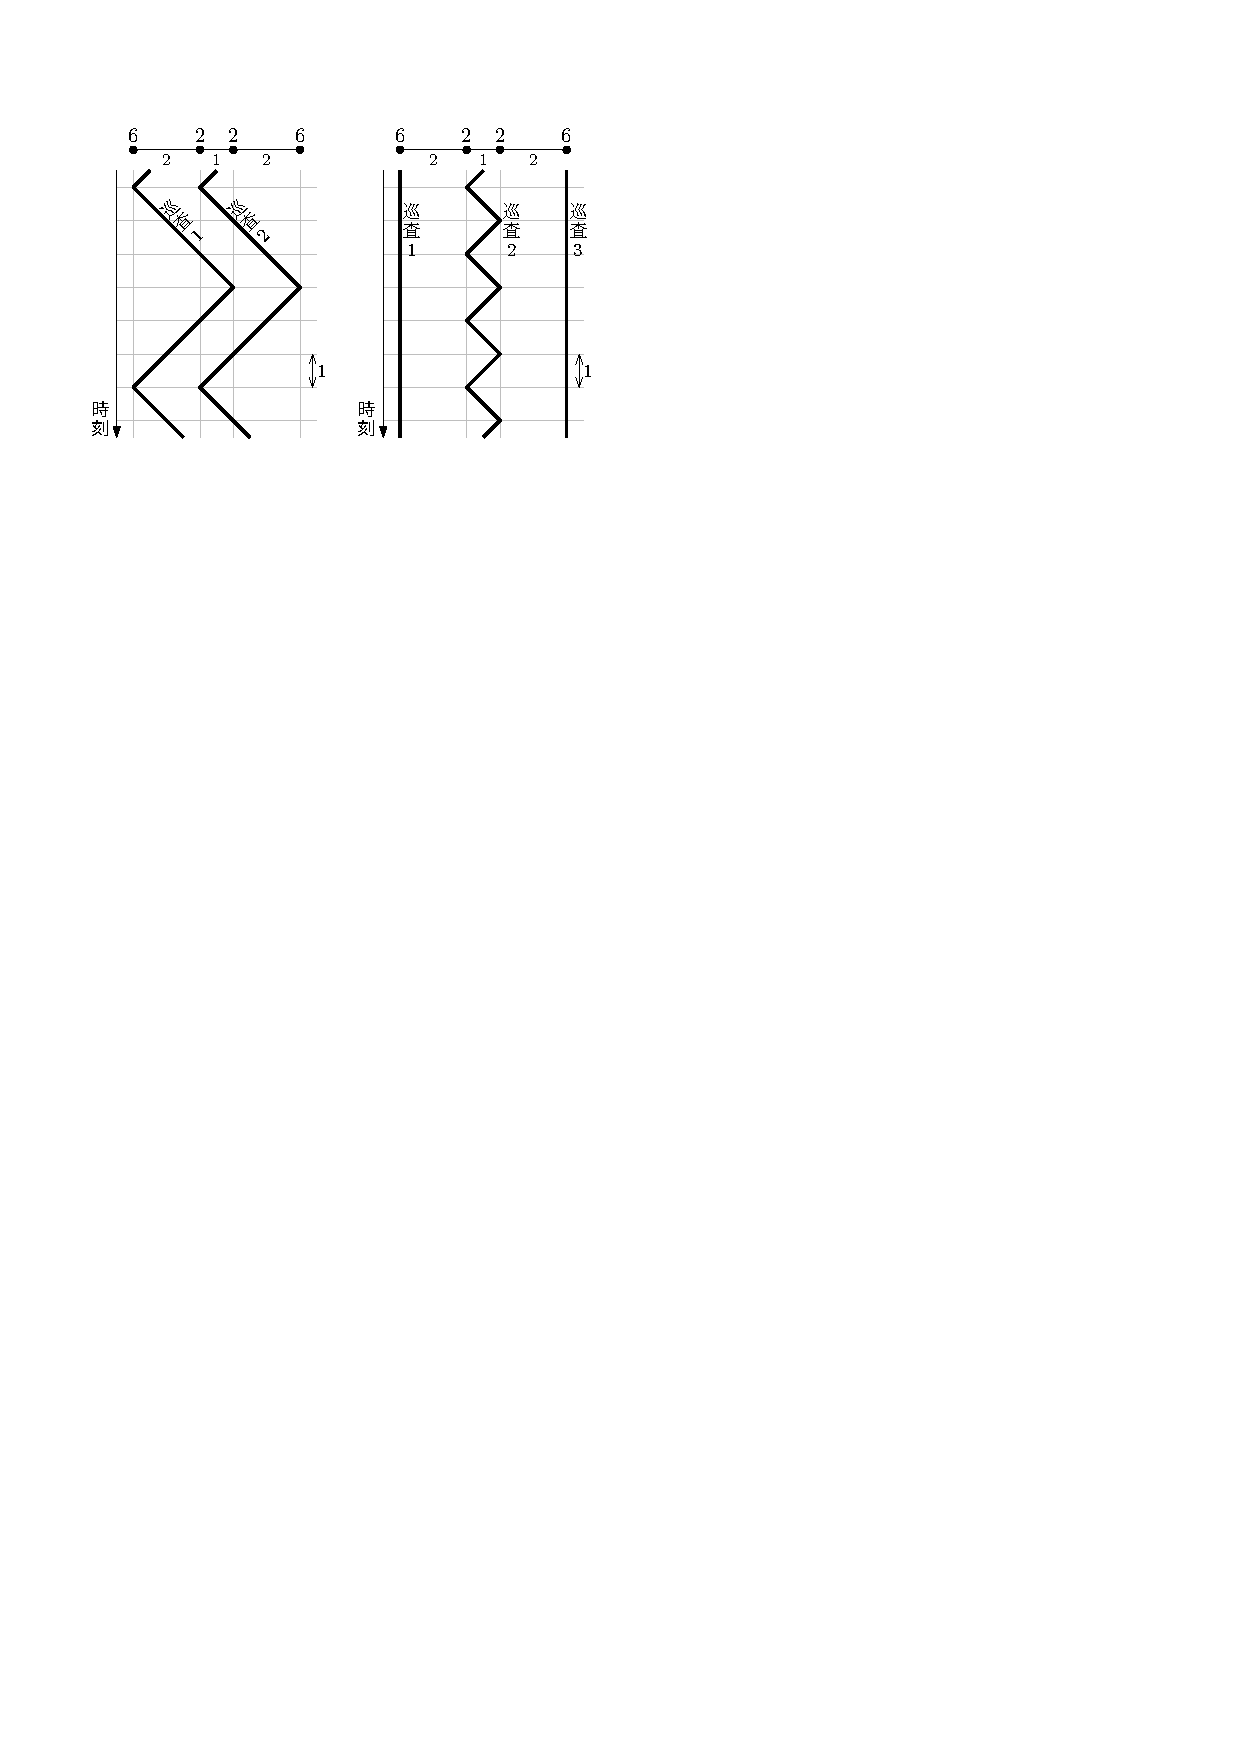
\includegraphics[scale=1.0]{\figdir/cooperative.pdf}
    \caption{図の上部に描かれている四点からなるグラフの全点を警邏する二つの運行.
      頂点と辺に書かれた数は,それぞれ{\idletime}と距離である.
      左図の運行では二人の巡査が協力して中央の二点を間隔$2$で警備している.
      これを禁じ,各点がいずれかの巡査により単独警備されることを求める場合は,
      右図のように三人の巡査を要する.}
    \label{figure: cooperative}
  \end{center}
\end{figure}
Coeneら\cite{coene2011charlemagne}は似た問題を扱っているが,
このような協力を許さず,
図\ref{figure: cooperative}右のように
各頂点を専ら一人の巡査が「担当」することを要求している.
つまり,各頂点$v \in W$が単独警備される(すなわち
或る一人の巡査がおり,
その巡査のみの運行が$\{v\}$を警邏する)ことを要求しているのである.
対比のため本稿ではこの問題を{\assignedPatProb}と呼ぶことにする
(\cite{coene2011charlemagne}ではMPLPPと称している).
Coeneら\cite{coene2011charlemagne}の諸結果においては,
この単独警備という限定が,
多項式時間算法の設計にも困難性の証明にも重要な役割を果している.
この限定を外したときの様子を調べるのが本稿の目的である.

本稿ではグラフの形状として
線分,星と,すべての枝の長さが等しい完全グラフの3種類を扱うこととし
(図\ref{figure: graph_classes}),
以降はそれぞれを {\graphLine}, {\graphStar}, {\graphUnit}と呼ぶ.
\begin{figure}
  \begin{center}
    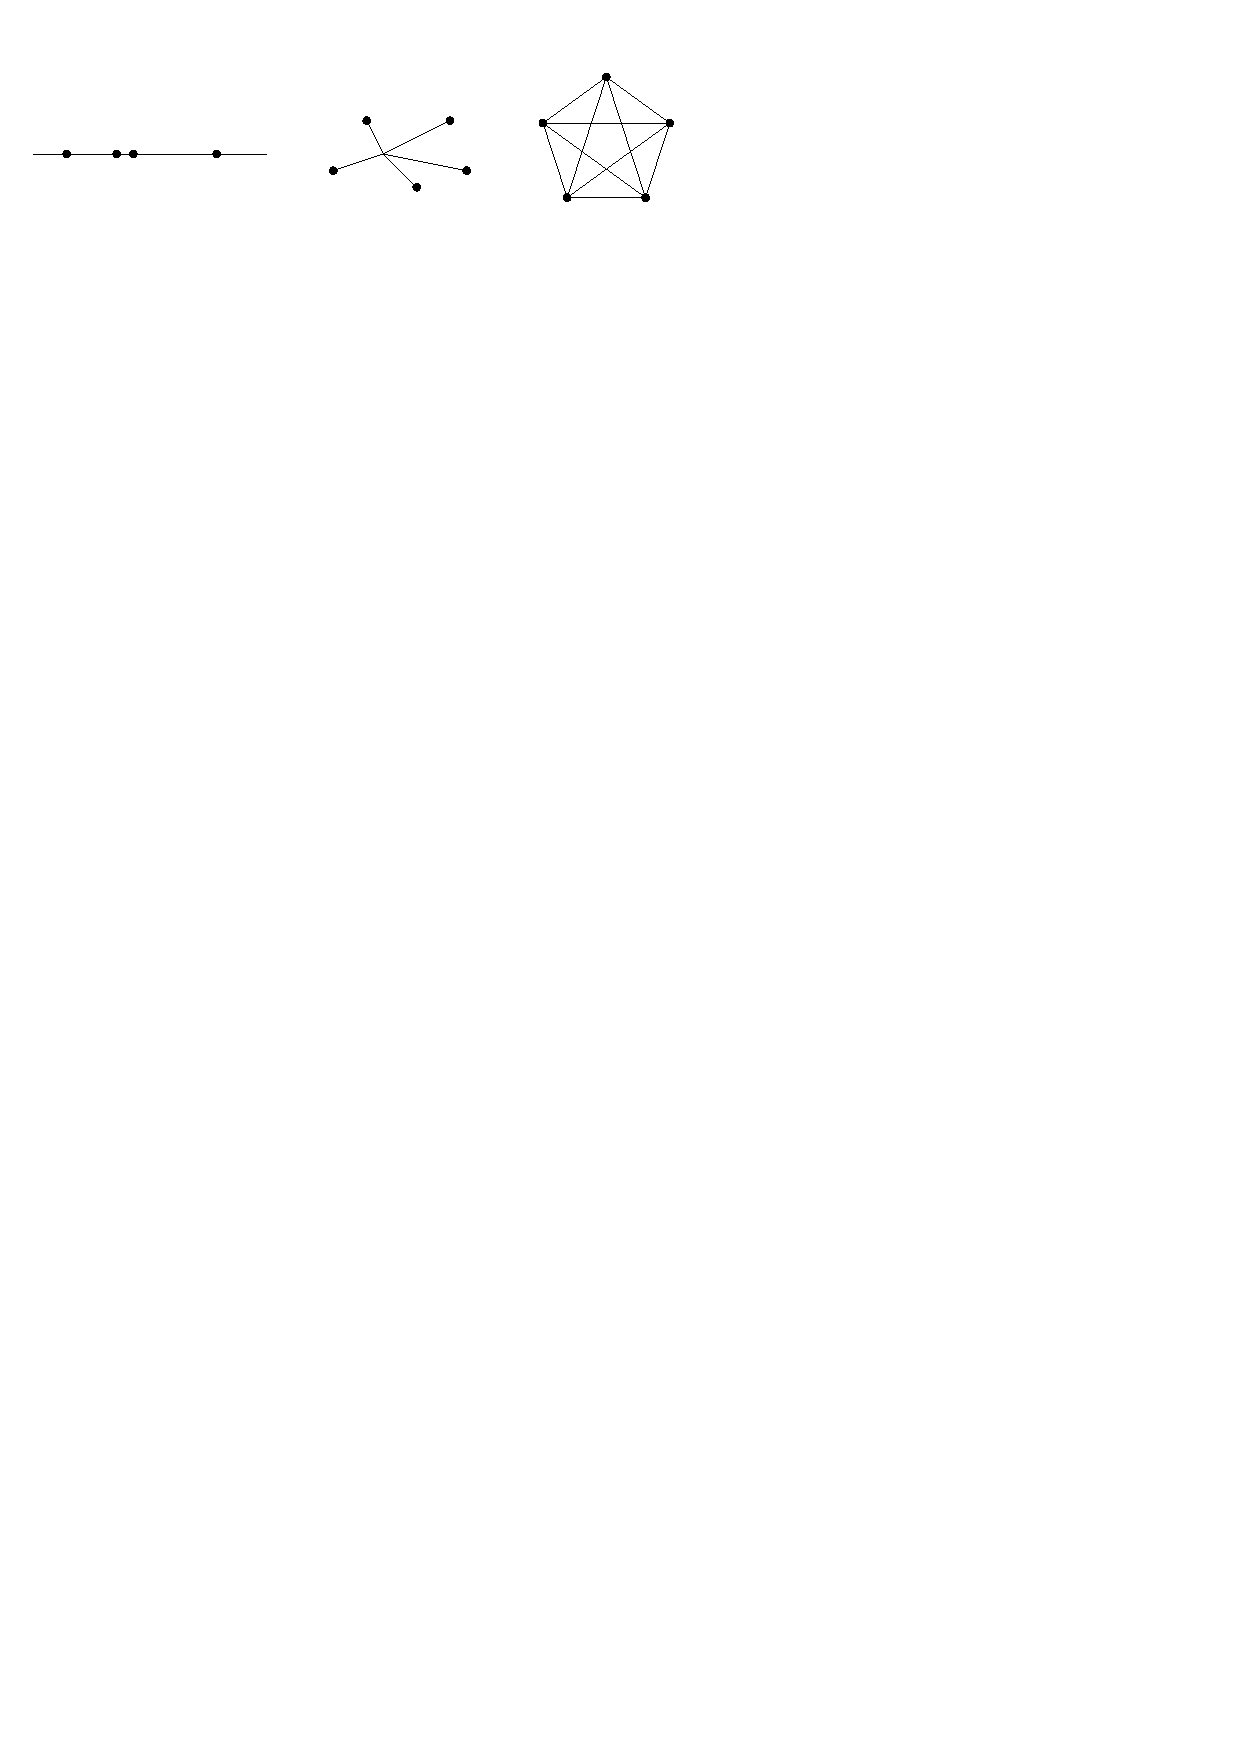
\includegraphics[scale=1.0]{\figdir/graph_classes.pdf}
    \caption{本論文では{\graphLine}(左),{\graphStar}(中),{\graphUnit}(右,但し各辺の長さが等しい)を扱う.{\graphStar}は葉のみを警備の対象とする(中央の点は移動の途中で使うのみであり,{\idletime}は定められていない).}
    \label{figure: graph_classes}
  \end{center}
\end{figure}
{\graphStar}では葉のみに{\idletime}が定められている(中心は警備の対象としない).
{\patProb}においては前述のとおり頂点同士の測地距離のみが重要であるため,
{\graphUnit}は,その各辺の長さを$d$とすると,
同じ頂点数で辺の長さがすべて$d/2$である{\graphStar}と同一視できることから,
{\graphUnit}は{\graphStar}の特殊な場合である.


% 巡査協力なしの結果との比較
{\patProb}についての我々の結果と,
{\assignedPatProb}についてのCoeneらの結果を,
グラフの形ごとに比較すると次のようになる.
それぞれ\ref{section: line},\ref{section: star},\ref{section: unit}節で述べる.
\begin{itemize}
  \item 
    グラフが{\graphLine}の場合は,
    {\assignedPatProb}は動的計画法により多項式時間で解けることが
    示されていた\cite[Theorem~11]{coene2011charlemagne}が,
    その正しさは非協力の設定に強く依存している.
    本稿では{\patProb}について,
    全点の{\idletime}が等しい場合には多項式時間で解ける
    (定理\ref{theo:LineEqualTimelimit}).
  \item
    グラフが{\graphStar}の場合は,
    全点の利得と{\idletime}が等しい場合に限っても,
    {\assignedPatProb}はNP困難であることが示されていた\cite[Theorem~10]{coene2011charlemagne}.
    本稿では,この場合の{\patProb}は多項式時間で解けるという興味深い結果を得る(定理**).
    なお利得または{\idletime}を一般にすると,
    巡査が一人であっても(したがって担当の有無に関わらず)
    NP困難であることがわかっている\cite[Theorems 5 and 6]{coene2011charlemagne}.
  \item 
    グラフが{\graphUnit}の場合は,
    全点の{\idletime}が等しい場合は{\patProb}が多項式時間で解けることを示す(定理**).
    グラフが{\graphStar}の場合は全点の{\idletime}が等しくても利得が一般だとNP困難になるので,
    これにより{\graphUnit}は{\graphStar}よりも簡単に解ける場合となっていることが分かる.
\end{itemize}


{\graphLine}と{\graphUnit}については
{\idletime}が一般の場合については多項式時間アルゴリズムやNP困難性を示すのが難しく未解決である.
これらの未解決な状況については,
{\idletime}の代わりに以下に定義する{\exactidletime}を警備の条件とする問題も考えた.

\begin{defi}
  運行$A = (a _1, \ldots, a _m)$が
  点$v \in U$を{\exactidletime}$(q, r)$で警備するとは,
  任意の時刻$t := q k + r (k \in \Zset)$に対し
  巡査$i$が存在し
  $a _i (t) = v$
  であることをいう.
\end{defi}

{\exactidletime}による{\patProb}は以下のように定義される.

\begin{timeSpecifiedCooperativePatrollingProblem}
  巡査の人数$m$と距離空間$U$内の点集合$V$および
  $V$の各点の利得と{\exactidletime}が与えられたとき,
  $m$人の巡査により警邏可能な頂点集合のうち利得の和が最大となるものを求めよ.
\end{timeSpecifiedCooperativePatrollingProblem}

判定問題は以下のようになる.

\begin{timeSpecifiedCooperativePatrollingProblemDecision}
  巡査の人数$m$と距離空間$U$内の点集合$V$および
  $V$の各点の{\exactidletime}が与えられたとき,
  $m$人の巡査により$V$を警邏可能か判定せよ.
\end{timeSpecifiedCooperativePatrollingProblemDecision}


{\graphLine}については{\timeSpecifiedPatProbDecision}を解く貪欲アルゴリズムを示す(定理\ref{}).
{\graphUnit}については{\timeSpecifiedPatProbDecision}がNP困難であることを示す(定理\ref{}).




\subsection*{関連研究}

\red{(あまり本筋に関係ない関連研究は、論文冒頭ではなくこの辺に書くのも手)}

% 警邏に関する研究には様々な問題設定があり,
% 例えば線分や閉路のような交わりの無い1次元的な領域のすべての点を警邏する
% 塀の警邏(Fence Patrolling)問題~\cite{chen2013fence, czyzowicz2011boundary}や,
% より一般的なグラフで辺全体ではなく頂点を警備する警邏問題~\cite{coene2011charlemagne},
% グラフと巡査が与えられて警邏可能かを判定する問題だけでなく,
% 塀の警邏問題においてなるべく長い塀を警邏する問題~\cite{czyzowicz2011boundary}や
% 全体の訪問の待ち時間の最大値を最小化する問題~\cite{chen2013fence}
% なども考えられている.
% \red{(加筆予定)}

また,{\graphLine}や{\graphStar}は木の特別な場合である.

\section{Line}
\label{section: line}

グラフがLineの場合,
グラフの全体(頂点と辺)をすべて実直線上におくことができる.
以降,頂点の名前$v_1, v_2, \ldots, v_n$はその位置を表す実数値も表すことにする.

まず,Lineの場合における順序保存運行という特別な運行を定義する.
運行$A$が順序保存であるとは,
$A$が定める巡査の位置$a_1, a_2, \ldots, a_m$が,
任意の時刻$t \in \Rset$において
$a_1(t) \leq a_2(t) \leq \cdots \leq a_m(t)$を満すことである.

Line上の任意の運行$A$は,$A$と同じ数の巡査でかつ警邏する点集合を保ったまま,
順序保存運行$A'$に以下のように変換することができる.
%
まず,$A$が定める各巡査の運行を$a_1, a_2, \ldots, a_m$とする.
これに対し,
$a'_i (i \in \mathset{1, \ldots, m})$を
各時刻$t \in \Rset$において$a' _i(t)$が
$a_1(t), a_2(t), \ldots, a_m(t)$のうち$i$番目に小さいものとなるように定める.
すると,各$a' _i$は運行となっており,
$A' = (a' _i)_{ i \in \mathset{1,\ldots, m} }$とすると
$A'$と$A$の運行の軌跡の集合は等しい
(すなわち,任意の時刻$t \in \Rset$において
$\mathset{a_1(t), \ldots, a_m(t)} = \mathset{a'_1(t), \ldots, a'_m(t)}$)
ので,
$A$で警邏していた点集合を$A'$も警邏している.
これにより順序保存運行$A'$が得られる.
%
順序保存運行$A'$は$A$において巡査がすれ違う時に代わりに
互いの動きを交換することにより順序を保ったものとみなすことができる.

以上から,
巡査$m$人により警邏可能な任意の頂点集合$W$は,
巡査$m$人による或る順序保存運行$A'$によって警邏されることが分かる.




%%%%% section 2.1 %%%%%

\subsection{全点の{\idletime}が等しい場合}
\label{subsec:LineUnaryTimelimit}




本節では次のことを示す.

\begin{theo}
  \label{theo:LineEqualTimelimit}
  グラフの形状がLineで全点の{\idletime}が等しい場合,
  {\patProb}は多項式時間で解くことができる.
\end{theo}

この問題は,~~な場合については Collinsら~\ref{}の問題の特殊な場合として既に示されているが,
ここでは全点の{\idletime}が等しいという条件のみでも成り立つことを示す.


以降では,
グラフの形状がLineで全点の{\idletime}が等しい場合,
警邏可能な頂点集合のうち利得の和が最大となるものは
次に定義する個別往復運行という運行によって警邏可能であるということを示す.
Lineで全点の{\idletime}が等しい場合に用いることができる
個別往復運行という戦略では
巡査の協力が不要になるため(補題\ref{lemm:LineEqualTimelimitIndependentInterval}),
全点の{\idletime}が等しいという条件が問題を簡単にしているといえる.


\begin{defi}
  $V$を頂点集合,$Q$を各頂点の{\idletime}とする.
  % $m$人の巡査による運行であって,
  % 各巡査が$V$のいずれかの頂点を左端とする長さ$Q/2$の区間を往復する運行を
  % $m$人の巡査による$V$上の個別往復運行と呼ぶ.
  各巡査が$V$のいずれかの頂点を左端とする長さ$Q/2$の区間を往復する運行を個別往復運行と呼ぶ.
  $m$人の巡査による運行$A$において各巡査が個別往復運行をしているとき,
  $A$を単に$m$人の巡査による個別往復運行と呼ぶ.
\end{defi}



まず次の補題を示す.

\begin{lemm}
  \label{lemm:RangeOfPatrollerOnLine}
  頂点$v_i$がある1人の巡査$s$により単独警備されているとき,
  {\idletime}を$q_i$として,
  $s$は常に区間$[v_i - q_i/2, v_i + q_i/2]$にいる.
\end{lemm}

\begin{proof}[証明]
  \newcommand{\vout}{v_{\mathrm{out}}}
  この区間にない或る座標$\vout \notin [v_i - q_i/2, v_i + q_i/2]$を$s$が
  時刻$t_0$に訪問するとする.
  $\vout$と$v_i$の間の移動には
  少くとも時間$\lvert v_i - \vout \rvert > q _i / 2$を要するから,
  $s$は区間$[t_0 - q _i / 2, t_0 + q _i / 2]$に属する時刻に$v_i$を訪問できない.
  この区間の長さは$
    q_i
  $であるので,$s$が$v _i$を単独警備していることに反する.
\end{proof}



これにより次の補題が成り立つ.


\begin{lemm}
 \label{lemm:LineEqualTimelimitIndependentInterval}
  グラフの形状がLineで,頂点の{\idletime}がすべて$Q$であるとする.
  頂点集合$W$が$m$人の巡査により警邏可能であるとする.
  このとき,
  $W$を警邏する$m$人の巡査による個別往復運行が存在する.
\end{lemm}


\begin{proof}[証明]

  \newcommand{\leftmostpoint}{b}  % v以外の記号
  \newcommand{\newpatroller}{l}
  \newcommand{\leftmostpatroller}{a_1}

  巡査数$m$に関する帰納法で示す.
  $m = 0$のときは明らかなので,以下$m > 0$とする.

  $W$は$m$人の巡査により警邏可能であるので,2章始めの議論により$W$を警邏する$m$人の巡査による順序保存運行が存在する.
  このような運行を任意に一つ選び
  $A = (a _i) _{i \in \{1, \ldots, m\}}$
  とする.

  $W$の点のうち最も左にあるものを$\leftmostpoint$とする.
  まず,各巡査は
  $\leftmostpoint$より左に存在する時間
  $\leftmostpoint$で停止するように変換する.
  このようにしても$W$は警邏されたままであり,
  また,これによりすべての巡査は
  $[\leftmostpoint, +\infty)$に存在することになる.

  ここで,最も左の巡査$\leftmostpatroller$に注目する.
  $\leftmostpoint$が$A$により訪問されるすべての時刻に
  $\leftmostpatroller$は$\leftmostpoint$を訪問しているので,
  $\leftmostpoint$は$\leftmostpatroller$により単独警備されている.
  %
  すると,
  補題\ref{lemm:RangeOfPatrollerOnLine}より,
  任意の時刻$t \in \Rset$に対し
  $\leftmostpatroller(t) \leq \leftmostpoint + Q/2$
  であるが,
  %
  一方,$\leftmostpatroller$は区間$[b, b + Q/2]$を速さ$1$で往復することで
  この区間に含まれるすべての頂点を警備することができる.
  実際,$\leftmostpatroller$がこのような往復をするとき
  $\leftmostpoint \leq x \leq \leftmostpoint + Q/2$
  である位置$x$に存在する時刻の間隔の最大値は
  \[
    \max( 2(x - \leftmostpoint), 2(\leftmostpoint + Q/2 - x) )
    \leq 2(\leftmostpoint + Q/2 - \leftmostpoint) = Q
  \]
  より,$[\leftmostpoint, \leftmostpoint + Q/2]$に含まれるどの頂点も
  {\idletime}を超えずに訪問できていることが分かる.
  これにより$\leftmostpatroller$の運行は個別往復運行となる.
  %
  一方,$W^- := \mathsetmid{ v \in W }{ \leftmostpoint + Q/2 < v }$は
  $\leftmostpatroller$以外の$m - 1$人の巡査により警備されているので,帰納法の仮定から
  残る$m - 1$人の巡査も個別往復運行に変換することができる.
  以上により$W$を警邏する$m$人の巡査による個別往復運行が得られた.
\end{proof}


補題\ref{lemm:LineEqualTimelimitIndependentInterval}により,
個別往復運行を行う場合のみを考えればよいため,
$m$人の巡査がそれぞれ担当する$m$個の区間を求めればよい.
以下のアルゴリズムにより利得の和が最大となる$m$個の区間を求めることができる.

初めにLine上の頂点をソートしておき,左側から順に$v_1,v_2,\ldots,v_n$とする.
頂点$v_i$を左端とする区間を$I_i := [v_i, v_i + Q/2]$と書く.

まず,
$n$個の区間$I_i (i = 1,2,\ldots, n)$について
各区間に含まれる点から得られる利得の合計$P_i$を求める.
$P_i$は$v_1,v_2,\ldots,v_n$がソートしてあるので$O(n)$で求めることができる.

あとは$m$個($m$は巡査の人数)の区間を選び利得の合計を最大化すればよいが,
以下の漸化式\ref{eq:LineWISPDP}に従う動的計画法で
$O(mn)$で
最大の利得を得られる$m$個の区間を選択できる.
$OPT(i,j)$は,区間$I_1, \ldots, I_j$から最大$i$個の区間を選ぶときの
利得の合計の最大値を表す.
$OPT(m,n)$が求めたい利得の最大値となる.
\begin{align}
  \label{eq:LineWISPDP}
  OPT(i,j) = 
  \begin{cases}
    0 & \text{$i = 0$または$j = 0$のとき} \\
    \max \{
      OPT(i, j - 1), 
      P_j + OPT(i - 1, j - 1)
    \}
    & \text{それ以外の場合}
  \end{cases}
\end{align}

最後に,$OPT(m,n)$において選ばれた区間をトレースバックして求め,
この区間に含まれる頂点全体を出力して終了する.

このアルゴリズムの計算量は全体で$O(n \log n + nm)$となる.
これで定理\ref{theo:LineEqualTimelimit}が示された.


% Circleについて
この証明では線分に端の頂点が存在することが重要な役割を果たしているため,
グラフの形状が閉路の場合にそのまま適用することはできない.


\subsection{{\idletime}が一般の場合}
\label{subsec:LineDifferentTimelimit}

全点の{\idletime}が等しい場合は
どの頂点も複数の巡査の協力で警備する必要がないため単純になっていたが,
{\idletime}が一般の場合は,
頂点を複数の巡査が交代で訪問して警備する必要がある場合が存在する.
%
図\ref{tikz:multiAgentExample2}(左)の例では,
中央の{\idletime}の短い2つの頂点を
2人の巡査が交互に訪問しており,
また,全点の{\idletime}が等しい場合と異なり
各巡査の最適な運行はなんらかの区間の往復であるとは限らないことも分かる.


また,
% \red{左から巡査の動きを決定できるのではないか?しかし,…
% ({\idletime}ぴったりの周期の場合についてのみ反例を作る?}
この例では左の巡査は左端の点を{\idletime}$10$ちょうどごとに訪問しているが,
左端の点の{\idletime}から順に巡査の運行を決定することも難しい次のような例が存在する.
図\ref{tikz:multiAgentExample2}(中央)の例では
{\idletime}$8$の左端の点をあえてより短い$6$ごとに訪問することで全点を警邏できるが,
同じグラフについて,
図\ref{tikz:multiAgentExample2}(右)のように左の巡査が
左端の点の{\idletime}ぎりぎりの時間まで右の方へ動き頂点をなるべく多くの時間訪問して左端へ帰る運行を選ぶと
右の巡査がどのような動き方をしても訪問間隔が{\idletime}を超え警備できない頂点が生まれてしまう.



\begin{figure}[h]
  \centering
  \begin{tabular}{ccc}

  \begin{minipage}{0.32\hsize}
    \centering
    \begin{tikzpicture}
      \draw [help lines,thin,step=5mm] (0,-5.0) grid (3.5,0);
      \draw[thick] (0,0) -- (3.5,0) node [below] {};
      \draw[thick, ->] (0,0) -- (0,-5.5) node [left] {$t$};

      \fill ( 0   , 0) coordinate (c1) circle (2pt) node [above] {10};
      \fill ( 1.5 , 0) coordinate (c2) circle (2pt) node [above] {2};
      \fill ( 2.0 , 0) coordinate (c3) circle (2pt) node [above] {2};
      \fill ( 3.5 , 0) coordinate (c5) circle (2pt) node [above] {10};

      \draw[very thick,- ] ( 1.0, 0  )--(   0,-1.0);
      \draw[very thick,- ] (   0,-1.0)--( 2.0,-3.0);
      \draw[very thick,- ] ( 2.0,-3.0)--( 1.5,-3.5);
      \draw[very thick,- ] ( 1.5,-3.5)--( 2.0,-4.0);
      \draw[very thick,->] ( 2.0,-4.0)--( 1.0,-5.0);

      \draw[very thick,- ] ( 2.0, 0  )--( 1.5,-0.5);
      \draw[very thick,- ] ( 1.5,-0.5)--( 2.0,-1.0);
      \draw[very thick,- ] ( 2.0,-1.0)--( 1.5,-1.5);
      \draw[very thick,- ] ( 1.5,-1.5)--( 3.5,-3.5);
      \draw[very thick,->] ( 3.5,-3.5)--( 2.0,-5.0);
    \end{tikzpicture}
  \end{minipage}

  \begin{minipage}{0.32\hsize}
    \centering
    \begin{tikzpicture}
      \draw [help lines,thin,step=5mm] (0,-4.5) grid (2.5,0);
      \draw[thick] (0,0) -- (2.5,0) node [below] {};
      \draw[thick, ->] (0,0) -- (0,-5) node [left] {$t$};

      \fill ( 0   , 0) coordinate (c1) circle (2pt) node [above] {8};
      \fill ( 1   , 0) coordinate (c2) circle (2pt) node [above] {2};
      \fill ( 1.5 , 0) coordinate (c3) circle (2pt) node [above] {2};
      \fill ( 1.75, 0) coordinate (c4) circle (2pt) node [above] {3};
      \fill ( 2.5 , 0) coordinate (c5) circle (2pt) node [above] {6};

      % \draw[very thick,red,<->] (1.75,-0.75)--(1.75,-2.25);

      \draw[very thick,- ] ( 0  , 0  )--( 1.5,-1.5);
      \draw[very thick,- ] ( 1.5,-1.5)--( 0  ,-3  );
      \draw[very thick,->] ( 0  ,-3  )--( 1.5,-4.5);
      \draw[very thick,- ] ( 1  , 0  )--( 2.5,-1.5);
      \draw[very thick,- ] ( 2.5,-1.5)--( 1  ,-3  );
      \draw[very thick,->] ( 1  ,-3  )--( 2.5,-4.5);
    \end{tikzpicture}
  \end{minipage}

  \begin{minipage}{0.32\hsize}
    \centering
    \begin{tikzpicture}
      \draw [help lines,thin,step=5mm] (0,-4) grid (2.5,0);
      \draw[thick] (0,0) -- (2.5,0) node [below] {};
      \draw[thick, ->] (0,0) -- (0,-5) node [left] {$t$};

      \fill ( 0   , 0) coordinate (c1) circle (2pt) node [above] {8};
      \fill ( 1   , 0) coordinate (c2) circle (2pt) node [above] {2};
      \fill ( 1.5 , 0) coordinate (c3) circle (2pt) node [above] {2};
      \fill ( 1.75, 0) coordinate (c4) circle (2pt) node [above] {3};
      \fill ( 2.5 , 0) coordinate (c5) circle (2pt) node [above] {6};

      \draw[very thick,red,<->] (1.75,-0.75)--(1.75,-2.25);

      \draw[very thick,- ] ( 0  , 0  )--( 1.5,-1.5);
      \draw[very thick,- ] ( 1.5,-1.5)--( 1  ,-2  );
      \draw[very thick,- ] ( 1  ,-2  )--( 1.5,-2.5);
      \draw[very thick,->] ( 1.5,-2.5)--( 0  ,-4  );

      \draw[very thick,- ] ( 1  , 0  )--( 2.5,-1.5);
      \draw[very thick,- ] ( 2.5,-1.5)--( 2.5,-2.5);
      \draw[very thick,->] ( 2.5,-2.5)--( 1  ,-4  );
    \end{tikzpicture}
  \end{minipage}

  \end{tabular}
  \caption{巡査の協力が必要な例.
    横軸を頂点の座標,縦軸を時刻として巡査の軌跡を表す.
    点の上の数値は{\idletime}を表す.
    \label{tikz:multiAgentExample2}}
\end{figure}




これらの例は,協力が発生する場合巡査の運行を個別に決定するのは難しいということを示唆している.
しかしながら,この{\idletime}が一般の場合でのLine上の{\patProb}の困難性を示すこともできなかった.
そこで,{\idletime}より短い間隔で点を訪問しうることで運行の決定を複雑になる例が存在したことを踏まえて,
1章で定義した時刻指定協力警邏判定問題を考える.




\begin{defi}
  $X \subset \Zset \times \Nset$とする.
  任意の$(t, x), (t', x') \in X$が
  $|t - t'| \geq |x - x'|$
  を満たすとき,$X$は運行可能であるという.
\end{defi}


任意の運行可能な集合$X$に対して,
Line上の巡査の運行$a$であって,
$X$のすべての元$(t, x)$に対して$a(t) = x$を満たすものが存在することは簡単に示すことができる.
これにより,
グラフがLineの場合の時刻指定協力警邏判定問題は次のようにも記述できる.

\begin{timeSpecifiedProblemOnLine}
  正の整数$m$(巡査の人数を表す)
  と自然数の組$(q_i, r_i, x_i)_{ i \in \{ 1, \ldots, n \} }$が与えられる.
  集合
  $\{ (q_i k + r_i, x_i) \mid i \in \{1, \ldots, n\}, k \in \Zset \}$
  を$m$個以下の運行可能な集合に分割できるか判定せよ.
\end{timeSpecifiedProblemOnLine}


% これを解くために次の副問題を考える.

% 1周期分だけ取り出して分割可能であることと元のXが分割可能であることが一致することを説明し
% アルゴリズムでは無限集合の周期的な分割を与えてYesかNoを答える
この問題では,
$X := \{ (q_i k + r_i, x_i) \mid i \in \{1, \ldots, n\}, k \in \Zset \}$
という無限集合の分割が可能か判定する必要があるが,
実際には$X$の点は時刻(組$(t, x) \in X$の第1要素)方向に周期的に並んでいるため,
その1周期分の有限部分集合を以下に定義する「周期的に運行可能な集合」に分割できるかどうかさえ
判定すればよい.

\red{理由を説明}

\begin{defi}
  $T$を正の整数,$X \subset \Zset \times \Nset$を有限集合とする.
  任意の$(t, x), (t', x') \in X$が
  $|t - t'| \geq |x - x'|$
  かつ
  $|t + T - t'| \geq |x - x'|$
  を満たすとき,$X$は周期$T$で繰り返し運行可能であるという.
\end{defi}


% \begin{timeSpecifiedProblemOnLineSubProb}
%   正の整数$m$
%   と自然数の組$(q_i, r_i, x_i)_{ i \in \{ 1, \ldots, n \} }$が与えられる.
%   集合
%   $X := \{ (q_i k + r_i, x_i) \mid i \in \{1, \ldots, n\}, k \in \Zset \}$
%   を$m$個以下の運行可能な集合に分割できるか判定し,
%   できるならば,
%   $T := lcm( q_1, \ldots, q_n )$とし,
%   有限集合
%   $\{ (t, x) \in X \mid 0 \leq t < T \}$
%   を周期$T$で繰り返し運行可能な$m$個以下の集合に分割せよ.
% \end{timeSpecifiedProblemOnLineSubProb}

% 明らかに時刻指定線分警邏問題は副問題に帰着できる.
% この副問題では上記のような$X$の分割が可能である場合には
% 必ず周期的な分割が存在することを主張している.
% % その1周期分の有限部分集合
% % $\{ (t, x) \in X \mid 0 \leq t < T \}$
% % の分割を与えることにより$X$全体の分割が可能であることを主張している.
% 実際に,この副問題は以下の貪欲アルゴリズムによって解くことができる.



% \begin{figure}[h]
%   \centering
%   \begin{tikzpicture}
%     \fill [fill=lightgray]
%       (1.5, -2)--(3.5,0)--(4,0)--(4,-4)--(3.5,-4)--(1.5, -2);
%     \draw[thick, ->] (0,0) -- (4.5, 0) node [below] {$x$};
%     \draw[thick, ->] (0,0) -- (0,-4) node [left] {$t$};

%     \fill ( 1.5,-2) coordinate (a) circle (2pt) node [left] {$(\alpha, \beta)$};

%     \node (L) at (1,-1.25) {$L(\alpha, \beta)$};
%     \node (R) at (3,-2) {$R(\alpha, \beta)$};
%   \end{tikzpicture}
%   \caption{$L(\alpha, \beta)$ と $R(\alpha, \beta)$ の定義 \label{tikz:defLR}}
% \end{figure}


\begin{greedyAlgorithmForTimeSpecifiedProblemOnLine}
  入力を$(m, (q_i, r_i, x_i)_{ i \in \{ 1, \ldots, n \} })$とする.
  始めに
  $T := lcm(q_1, \ldots, q_n)$,
  $X := \{ (q_i k + r_i, x_i) \mid i \in \{1, \ldots, n\}, k \in \Zset \}$,
  $L((\alpha, \beta)) := \{(t, x) \mid x - \beta \leq |t - \alpha| \}$と記号を定義する.

  まず$X$の部分集合$S := \{ (x, t) \in X \mid -T \leq t < 2T \}$を求める.
  初期値を$\mathcal{B} = \{\}$, $B_0 = S$, $B' = S$, $i = 0$とし,
  $B_i \neq \emptyset$である限り1.から4.を繰り返す.
  \begin{enumerate}
    \item $i \gets i + 1$, 
    \item $B_i \gets B' \cap \left( \bigcap_{p \in B'} L(p) \right)$, 
    \item $B' \gets B' \setminus B_i$, 
    \item $\mathcal{B} \gets \mathcal{B} \cup \{ B_i \}$.
  \end{enumerate}

  $|\mathcal{B}| > m$ならば分割不可能と答え,
  そうでないときは分割可能と答えたうえで,
  $\mathcal{B}$の各元を時刻方向に$[0, T)$に制限したもの
  $\mathcal{C} := \{ \{ (t, x) \in B \mid 0 \leq t < T \} \mid B \in \mathcal{B} \}$
  を出力して終了する.
\end{greedyAlgorithmForTimeSpecifiedProblemOnLine}

% 副問題は主問題の判定を行いさらに繰り返し運行可能分割を求める問題なので,
% 主問題の判定ができていることをここで説明する必要がある.
この貪欲アルゴリズムが
\begin{itemize}
  \item 分割不可能と答えるとき,
    $X$も$m$個の運行可能な集合に分割することはできない.
    実際,
    $X$が$m$個の運行可能な集合に分割できるとき,
    $S := \{ (x, t) \in X \mid -T \leq t < 2T \}$
    は$X$の部分集合であるから$m$個の運行可能な集合に分割できるが,
    その場合は貪欲アルゴリズムは必ず$m$個の運行可能な集合への分割を答える.
    これは次の理由による.
    Lineにおいては順序保存運行の存在と同様に,
    $S$が$m$個の運行可能な集合へ分割可能ならば
    $S$の$m$個の運行可能な集合への分割であって順序保存なものが存在する.
    ここで,分割$\mathcal{B'} = \{ B'_1, \ldots, B'_m \}$が順序保存であるとは,
    対応する運行$(b_1, \ldots, b_m)$が順序保存運行になることである.
    貪欲アルゴリズム中で得られる$S$の分割$\mathcal{B} = \{ B_1, \ldots, B_m \}$は
    任意の順序保存な$S$の分割を選び$\mathcal{B'} = \{ B'_1, \ldots, B'_m \}$と整数$k$に対し,
    $\bigcup_{1 \leq i \leq k} B'_i \subseteq \bigcup_{1 \leq i \leq k} B_i$
    を満たしており,これにより
    $S$が$m$個の運行可能な集合へ分割可能ならば
    貪欲アルゴリズムは必ず$m$個の運行可能な集合への分割を答えることが分かる.
  \item 分割可能と答えるとき,
    $X$も$m$個の運行可能な集合に分割することができる.
    実際,
    分割可能と答えるときには分割$\mathcal{C}$を出力するが,
    $\mathcal{C}$の各元$C$は
    周期$T$で繰り返し運行可能な集合である.
    これは,途中の各$B \in \mathcal{B}$が$L$の定義から運行可能集合となっており,
    $B$の$[-T, 2T)$の範囲が運行可能であれば$[0, T)$の範囲は
    定義から周期$T$で繰り返し運行可能となるためである.

    集合
    $X := \{ (q_i k + r_i, x_i) \mid i \in \{1, \ldots, n\}, k \in \Zset \}$
    の分割$\mathcal{A} = \{ A_1, \ldots, A_m \}$は次のように構成すればよい.
    $k \in \Zset$に対して,$X$の部分集合
    $\{ (t, x) \in X \mid kT \leq t < (k + 1)T \}$
    を$\mathcal{C}$の分割の仕方で分割したものを$\{ C_{k1}, \ldots, C_{km} \}$とする.
    $A_i := \bigcup_{k \in \Zset} C_{ki}$と定義すると,
    $C_{ki}$が周期$T$で繰り返し運行可能な集合であるから,
    $A_i$は運行可能な集合となる.
    % $\mathcal{A}$は$X$を$m$個の運行可能な集合へ分割したものとなっている.
\end{itemize}
以上より,貪欲アルゴリズムは副問題を解く.





% 三角形領域$R(t_a, x_a)$は,
% 時刻$t_a$に$x_a$に存在する巡査が存在し得ない位置と時刻の組の集合のうち
% $x_a$より右側の領域を表している($|x - x_a| / |t - t_a| > 1$かつ$x_a < x$).
% 訪問しなければならない位置と時刻の組の集合$X$に対して,
% $\dbigcap_{a \in X} L(a)$は
% 一番左の巡査の存在可能領域を表す(補題**).



% 本節で示すのは以下の定理である.
% \begin{theo}
%   \label{lemm:LineExactFinite}
%   グラフの形状がLineのとき,
%   時刻指定{\patProb}は,
%   「最右運行」で巡査の運行を左端から順に決定する\red{(←手順が未定義)}ことで
%   全点警邏可能か判定できる.
%   % \red{
%   %   指定時刻が有限個ならその個数の多項式時間で判定できる、とかにする?
%   %   入力が周期と剰余なら$O(*)$で計算できる、とかに?
%   % }
% \end{theo}


% \begin{lemm}
%   \label{lemm:leftmostAgentExistableTerrain}
%   $X$を訪問しなければならない位置と時刻の組の集合とする.
%   このとき,
%   順序保存運行において一番左の巡査$s$の軌跡は
%   $\bigcap_{a \in X} L(a)$に含まれる.
% \end{lemm}

% \begin{proof}
%   巡査$s$の軌跡に$\bigcup_{a \in X} R(a)$の点$b = (t_b, x_b)$が含まれるとすると,
%   ある$a = (t_a, x_a) \in X$が存在して$b \in R(a)$となる.
%   巡査の速さは1以下なので時刻$t_a$における巡査$s$の位置$x$は
%   $|x_b - x| \leq |t_b - t_a|$を満たすが,
%   $b \in R(a)$より$x_b - x_a > |t_b - t_a|$なので
%   $x_b - x \leq |x_b - x| < x_b - x_a$,
%   すなわち$x_a < x$となる.
%   $x_a < x$より$x_a$を警備する$s$より左の巡査が必要になり矛盾する.
%   よって,$s$の軌跡は$\bigcup_{a \in X} R(a)$の点を含まない.
% \end{proof}

% これにより次がいえる.

% \begin{lemm}
%   \label{lemm:LineExactFinite}
%   グラフ$G$がLine,指定時刻全体が$X$のときの時刻指定{\patProb}において,
%   $m$人の巡査により$G$を警邏可能であるとき,
%   $m$人の巡査のうち
%   $1$人の巡査が$X$に対する最右運行であるような運行により$G$を警邏できる.
% \end{lemm}

% \begin{proof}
%   指定時刻の集合を$X$とする.
%   $G$は$m$人の巡査により警邏可能であるので,
%   2章始めの議論により$G$を警邏する$m$人の巡査による順序保存運行が存在する.
%   このような運行を任意に一つ選び$A = (a_1, \ldots, a_m)$とする.
%   補題\ref{lemm:leftmostAgentExistableTerrain}より
%   $A$における一番左の巡査の運行$a_1$の軌跡は
%   $\bigcap_{a \in X} L(a)$に含まれる.
%   $\bigcap_{a \in X} L(a)$に含まれる$X$の点は$b(X)$上に存在するので
%   $a_1$の軌跡に含まれる$X$の点は$b(X)$に含まれる.
%   一方,$b(X)$は傾きが$\pm 1$の線分からなる連続な領域なので
%   一番左の巡査は$b(X)$が軌跡となる運行$a_1'$を行うことができ,
%   $b(X)$上のすべての点を訪問できる.
%   定義より$a_1'$は最右運行であり,
%   $A$において運行$a_1$を$a_1'$に替えた運行$(a_1', a_2, \ldots, a_m)$もやはり$G$を警邏している.
% \end{proof}

% % 全点を警備する任意の順序保存運行$A$で一番左側を動く巡査$s_1$の軌跡を考える.
% % %
% % もし$t$-$x$平面上のある点$(t_a,x_a)$から定まる$R(t_a,x_a)$に含まれる点$(t',x')$を
% % $s_1$の軌跡が通っているとすると,
% % $s_1$は$|x_a - x'| > |t_a - t'|$より時刻$t_a$に座標$x_a$を訪問できないので
% % $s_1$が一番左側を動くことから$(t_a,x_a)$が訪問されない点となってしまい矛盾する.
% % %
% % よって,$A$で一番左側を動く巡査$s_1$の軌跡は$\dbigcap_{a \in X'} L(a)$に含まれる.
% % $L(X') := \dbigcap_{a \in X'} L(a)$とする.

% % 一方,この領域$L(X')$の境界線は傾き$1$または$-1$の線分のつながったものであるので,
% % $s_1$はこの境界線が軌跡となるように動くことができ,
% % そのようにすることで$L(X')$に含まれるすべての点を訪問でき
% % $A$での$s_1$の動きを改善できる.
% % %
% % $s_2, s_3, \ldots, s_m$の動き方も$X'$ の残りの点に対して
% % $s_1$のときと同様に決めていくことで$A$での動きを改善できる.


\section{Star}
グラフの形状がStarの場合については,
利得か{\timelimit}のいずれかが一般であれば,
{\patrolling}は巡査が1人であってもNP困難であることがわかっている\cite{coene2011charlemagne}.
そこで,ここでは巡査数が一般であって,
利得と{\timelimit}がすべて等しい場合を考える.
%
この場合,非協力警邏問題ではNP困難になることが
Coeneら\cite{coene2011charlemagne}により示されているが,
今回考えている協力警邏問題では多項式時間で解くことができる.
%
これは,
非協力の場合にはうまく分担する方法を見つける必要があるのに対し,
協力警邏の場合には単純で最適な警邏を構成できることが理由となっている.

以下では
% そのような単純な警邏の仕方を示していくが,
{\timelimit}を$Q$とするとき,
「複数人の巡査が間隔$Q$ずつ離れて列を成し巡回する」動き
と「点に1人の巡査が常駐する」という2種類の運行の組合せで
最適な運行が得られることを示す.

% 隣接枝が一定以上長い点は
% 枝の往復にかかる時間が大きくなるため,
% 巡回に含めずに巡査を1人常駐させる方が
% この点の1回あたりの警備にかかる時間を減らすことができる.



\begin{theo}
    \label{theo:StarEqualProfitTimelimit}
    グラフの形状がStarで利得と{\timelimit}がすべて等しい場合,
    {\patrolling}は多項式時間で解くことができる.
\end{theo}


\begin{proof}[証明]

    巡査数を$m$, 全頂点の{\timelimit}を$Q$, 
    頂点$v_i (i \in \mathset{1,\ldots, n})$に隣接する枝を$e_i$, その長さを$d_i$とする.
    枝の長さは$d_1 \leq d_2 \leq \cdots \leq d_n$であるとする.

    まず,
    すべての頂点の利得と{\timelimit}が等しいので,枝の短い頂点から選べばよいことが分かる.
    実際,ある警邏において警備している頂点$v_i$と警備していない頂点$v_j$であって
    隣接枝$e_i$, $e_j$の長さが$d_i > d_j$となっているようなものがあったとき,
    $v_j$を訪問していた時刻に代わりに$v_i$を訪問するようにすべての巡査の動きを変えることができる.




    まず,$d_i > Q/2$であるような頂点$v_i$は,警備するならば巡査が1人常駐するとしてよい.
    これは次のように示される.
    %
    (i)ある運行において$v_i$が1人の巡査$s$により単独警備されるとすると,
    $v_i$を訪問してから別の頂点$v_j$を訪問して再び$v_i$に戻ってくるには$2d_i$以上の時間がかかり
    $2d_i > Q$より$v_i$が警備できなくなってしまうため$v_i$以外の頂点を警備することができないので
    $v_i$のみを警備すればよく,これは$v_i$に常駐すれば十分である.
    %
    (ii)もし$v_i$が2人以上の巡査により警備されるとすると,
    ある巡査$s_a$が時刻$t_a$に$v_i$を訪問してから時間$Q$以内の時刻$t_b$に
    別の巡査$s_b$が$v_i$を訪問するという状況が発生するが,
    $s_a$が枝
    $s_b$は端点$v_i$を含む枝$e_i$上のある点に同時に存在するような時刻が
    $s$が
    $s$は$s'$とすれ違うことなく$v_i$以外の頂点を訪問



    2人の巡査がすれ違う動きは互いに動きを交換して引き返す動きに変換しているとすると
    $s$と$s'$が枝$e_i$上で1度以上すれ違わない限り$s'$が$v_i$を訪問するときには$s$も
    $v_i$を訪問しているので,
    $v_i$は$s$のみにより警備できており,$s$も$v_i$以外を警備していない動きとなる.



    よって,あとは隣接している枝の短い頂点から何個の頂点を選べるかを計算できればよい.
    %
    はじめに,頂点を枝の長さの昇順でソートし,枝の短いものから順に$v_1,v_2, \ldots, v_n$とする.
    これらを枝の長さが$Q/2$以下のグループ$V_1 = \mathset{v_1, \ldots, v_k}$と
    それ以外のグループ$V_2 = \mathset{ v_{k + 1}, \ldots, v_n }$に分ける.
    $V_2$の頂点は,$V_1$の全頂点を$m - 1$人以下の巡査により警備できる場合のみ,
    残りの巡査の人数分$V_2$の頂点を選び1人ずつ巡査を常駐させることで警備すればよいので,
    まず$V_1$のすべての頂点を警備できる最小の巡査数$m'$を求める必要がある.

    $m' \leq m$であれば利得(警備できる頂点数)は$k + (m - m')$となる.
    $m' > m$であれば$V_1$のうち

\end{proof}


\section{{\graphUnit}}
\label{section: unit}

第1章で述べた通り,{\graphUnit}は{\graphStar}の特殊な場合とみなせるため,
定理\ref{theo:StarEqualProfitTimelimit}から
全点の利得と{\idletime}が等しい場合は
{\patProb}を多項式時間で解くことができるが,
{\graphUnit}の場合は全点の{\idletime}だけが等しければ{\patProb}を多項式時間で解ける
(定理\ref{theo:UnitEqualTimelimit}).

{\idletime}が一般の場合については
多項式時間アルゴリズムやNP困難性を示すのが難しかったため,
第2章で扱った{\timeSpecifiedPatProb}を再び考える.
グラフが{\graphUnit}の場合は{\timeSpecifiedPatProb}がNP困難になることを示す
(定理\ref{theo:unit_exacidletime_NPhard}).



\subsection{全点の{\idletime}が等しい場合}

\begin{theo}
  \label{theo:UnitEqualTimelimit}
  グラフの形状が{\graphUnit}で全点の{\idletime}が等しい場合,
  {\patProb}は(利得,巡査数が一般であっても)多項式時間で解くことができる.
\end{theo}

\begin{proof}
  補題\ref{lemm:condition_of_guarding_star}から
  {\graphUnit}の全点の{\idletime}が$Q$のとき,
  点集合$V$の任意の部分集合$W$について
  $$
    \sum_{v \in W} \min(d, Q) = \card{W}\min(d, Q) \leq mQ
    \iff \text{$m$人の巡査により$W$の全点を警邏できる}
  $$
  が成り立つ.$d$は{\graphUnit}の各辺の長さである.

  グラフの形状が{\graphUnit}の場合,
  全点の{\idletime}が等しいならば警邏する部分集合$W$は利得の大きい点から選べばよい
  (利得のより大きい点$v_1$とより小さい点$v_2$があるとき,
  $v_1$を警備して$v_2$を警備しない運行は常に$v_1$を警備する代わりに$v_2$を警備する運行に変換できる).
  $\card{W}\min(d, Q) \leq mQ$を満たす最大の$\card{W}$は
  $\card{W} = \left\lfloor {mQ}/{\min(d, Q)} \right\rfloor$
  であり,利得の大きい点から$\lfloor {mQ}/{\min(d, Q)} \rfloor$点を選ぶ計算は
  $O(\lfloor {mQ}/{\min(d, Q)} \rfloor \log n)$となる.
\end{proof}




\subsection{{\idletime}が一般の場合:{\timeSpecifiedPatProb}}


\begin{theo}
  \label{theo:unit_exacidletime_NPhard}
  グラフの形状が{\graphUnit}のとき,
  {\timeSpecifiedPatProb}は巡査が1人で全点の利得が等しくてもNP困難である.
\end{theo}

% 最大独立集合問題において,
% 無向グラフが与えられたときに独立点集合で最大のものを求めるが,
% 間に辺の存在する2頂点の両方を選ぶことはできないという制約を,
% {\patProb}において2頂点のどちらか一方しか警備できないという制約に変換する.

\begin{proof}[証明]
  最大独立集合問題からの帰着による.

  最大独立集合問題の入力のグラフが$G = (V, E)$のとき,
  {\timeSpecifiedPatProb}に対して,
  巡査の人数$1$と{\graphUnit}のグラフ$G' = (V', E')$を入力として与える.
  $G'$は以下のように定める.
  $V' = V$とし,全点の利得は$1$,辺の長さはすべて$1$とする.
  各点の{\exactidletime}は次のように定める.
  %
  まず,${}_n C_2$ 個の相異なる素数 $p_{i,j} (1 \leq i < j \leq n)$ を用意し,
  $q_i := \prod_{k = 1}^{i - 1} p_{1,k} \prod_{k = i + 1}^n p_{k,n}$
  とする.
  次に,$r_i (i \in \{1, \ldots, n\})$を,
  $G$のすべての2点$v_i, v_j (1 \leq i < j \leq n)$に対して,
  $(v_i, v_j) \in E$     ならば $r_i \equiv    r_j \equiv 0 \mod p_{i,j}$,
  $(v_i, v_j) \not\in E$ ならば $r_i \equiv 0, r_j \equiv 1 \mod p_{i,j}$,
  さらに$0 \leq r_i < q_i$
  を満たすように定める.
  各$r_i$に対して相異なる$n - 1$個の素数で割ったときの余りが与えられているので,
  中国剰余定理からそのような$r_i$がその$n - 1$個の素数の積$q_i$を法として一意に存在する.
  %
  以上のようにして得た$q_i, r_i (i \in \{ 1, \ldots, n\})$から,
  各点$v_i (i \in \{1, \ldots, n\})$の{\exactidletime}を$q_i k + r_i (k \in \Nset)$
  と定めると,
  {\timeSpecifiedPatProb}の解は$G$の最大独立集合となる.

  実際,
  $G'$の任意の2点$v_i$, $v_j$($i < j$としてよい)に対し,
  この両方を警備できるための必要十分条件は,
  2点間の移動時間が$1$以上かかることから,
  訪問しなければならない時刻同士がすべて$1$以上離れていること,すなわち,
  任意の整数$k, l$に対し$\abs{(k q_i + r_i) - (l q_j + r_j)} \geq 1$
  が成り立つこととなる.
  $q_i, r_i, q_j, r_j$がすべて整数のとき,これは
  $q_i k + r_i \neq q_j l + r_j$, 
  すなわち
  $r_i - r_j \neq q_j l - q_i k$
  が任意の整数$k, l$で成り立つこと同値である.
  $gcd(x,y)$を$x$と$y$の最大公約数とすると,
  $r_i - r_j \neq gcd(q_i,q_j) n$が任意の整数$n$で成り立つこと,
  つまり$r_i \not\equiv r_j \mod gcd(q_i, q_j) = p_{i,j}$と同値である.
  よって,
  $v_i$ と $v_j$ の両方を警備できる必要十分条件は
  $r_i \not\equiv r_j \mod p_{i, j}$
  となる.
  $r_i$の決め方から,
  \[
    (v_i, v_j) \in E \iff \text{$G'$の2点$v_i, v_j$を両方警備することができない}
  \]
  が成り立つため,
  $G'$の点部分集合であって同時に警備できない2点のうち少なくとも一方は含まないようなもののうち
  最大のものを選ぶと,
  これは$G$の最大独立集合となる.

  最後に,${}_n C_2$ 個の相異なる素数を用意する計算量も確かめる必要がある.
  $k$ 番目に小さい素数を $P_k$ と書くと,$k \geq 6$ のときは
  $P_k < k( \ln k + \ln\ln k )$ であることが知られているため~\cite{dusart1999k},
  $k( \ln k + \ln\ln k )$ までの自然数を順に素数かどうか判定していくことで
  $k$ 個以上の素数を得ることができる.
  ある数が素数であるかどうかを判定する多項式時間アルゴリズムは存在するので~\cite{agrawal2004primes},
  ${}_n C_2$ 個の素数の列挙は$n$の多項式時間でできる.
\end{proof}



定理\ref{theo:unit_exacidletime_NPhard}では,
各点の{\exactidletime}といっても間隔$q_i$と剰余$r_i$が与えられる場合について
NP困難性が示したが,
各点に間隔$q_i$のみが指定されている
「{\intervalSpecifiedPatProb}」も考えることができる.
これの全点警邏判定問題を「{\intervalSpecifiedPatProbDecision}」と呼ぶことにする.

\begin{theo}
  \label{theo:NPhard_disjoint_residue_class_problem}
  グラフの形状が{\graphUnit}のとき,
  {\intervalSpecifiedPatProbDecision}は巡査が1人であってもNP困難である.
\end{theo}


\begin{proof}[証明]
  Disjoint Residue Class Problem~\cite{kawamura2015simple}からの帰着による.

  ある整数の組の集合 $\{ (m_1, r_1), \ldots, (m_n, r_n) \}$ が
  Disjoint Residue Class であるとは,
  任意の整数 $x$ に対して $x \equiv r_i \mod m_i$ となるような $i$ が
  高々1つ存在することと定義される.
  Disjoint Residue Class Problem とは
  整数の組 $(m_1, \ldots, m_n)$ が与えられたときに,
  $\{ (m_1, r_1), \ldots, (m_n, r_n) \}$ が
  Disjoint Residue Class となるような組 $(r_1, \ldots, r_n)$ が
  存在するかを判定する問題であり,
  NP困難であることが知られている~\cite{kawamura2015simple}.

  Disjoint Residue Class Problem の入力が $(m_1, \ldots, m_n)$ のとき,
  {\intervalSpecifiedPatProb}に対して
  巡査の人数$1$と$n$点からなる{\graphUnit}のグラフで
  各点の{\exactinterval}を$q_i = m_i$となるように定め,辺の長さはすべて$1$としたものを
  入力として与えることで
  Disjoint Residue Class Problemを解くことができる.

  辺の長さが$1$であるから,すべての整数の時刻にいずれかの1点を訪問できる.
  各頂点$v_i$の最初の訪問時刻\red{←替える}を$r_i$とすると,
  この点を警備するために訪問しなければならない時刻の列は
  $q_i k + r_i (k \in \Nset)$で与えられるが,
  全点を警備するためには任意の2点$v_i, v_j \in V$, 任意の整数$k,l$について
  $q_i k + r_i \neq q_j l + r_j$
  である必要がある.

  Disjoint Residue Class Problem の解 $(r_1, \ldots, r_n)$ が存在するならば,
  任意の時刻 $t \in \Zset$ に対して $t \equiv r_i \mod q_i$, 
  すなわち $t = r_i + q_i k$ となる $k \in \Zset$ が存在するような $i$ は高々1つであり,
  任意の $k,l \in \Zset$ に対して $q_i k + r_i \neq q_j l + r_j$ が成り立つので,
  巡査は全点を警備でき,
  解が存在しなければ
  あるの整数$x$に対して $x \equiv r_i \mod m_i$, $x \equiv r_j \mod m_j$
  となる$i, j$が存在するので,
  $v_i, v_j$を両方警備することができず,したがって全点を警備できない.
\end{proof}



\begin{thebibliography}{1}

%\bibitem{agrawal2004primes}
%M. Agrawal, N. Kayal, and N. Saxena.
%\newblock Primes is in P.
%\newblock {\em Annals of Mathematics}, 160(2), pp. 781--793, 2004.

\bibitem{chen2013fence}
K.~Chen, A.~Dumitrescu, and A.~Ghosh.
\newblock On fence patrolling by mobile agents.
\newblock In {\it Proc.\ 25th Canadian Conference on Computational Geometry} (CCCG), 2013.


%\bibitem{coene2013balancing}
%S.~Coene, C.~Filippi, F.\,C.\,R. Spieksma, and E.~Stevanato.
%\newblock Balancing profits and costs on trees.
%\newblock {\em Networks}, 61(3), pp.~200--211, 2013.


\bibitem{coene2011charlemagne}
S.~Coene, F.\,C.\,R.~Spieksma, and G.\,J. Woeginger.
\newblock Charlemagne's challenge: the periodic latency problem.
\newblock {\em Operations research}, 59(3), pp.~674--683, 2011.


\bibitem{czyzowicz2011boundary}
J.~Czyzowicz, L.~G{\k{a}}sieniec, A.~Kosowski, and E.~Kranakis.
\newblock Boundary patrolling by mobile agents with distinct maximal speeds.
\newblock In {\it Proc.\ 19th Annual European Symposium on Algorithms} (ESA), LNCS~6942, pp.~701--712, 2011. 


%\bibitem{dusart1999k}
%P.~Dusart.
%\newblock The $k$th prime is greater than $k (\ln k + \ln \ln k - 1)$ for $k \geq 2$.
%\newblock {\em Mathematics of Computation}, 68, pp.~411--415, 1999.


\bibitem{kawamura2015simple}
A.~Kawamura and M.~Soejima.
\newblock Simple strategies versus optimal schedules in multi-agent patrolling.
\newblock In \emph{Proc.\ Ninth International Conference on Algorithms and Complexity} (CIAC), LNCS~9079, pp.~261--273, 2015.

\end{thebibliography}



\end{document}
